\documentclass[10pt,xcolor={dvipsnames}, aspectratio=169]{beamer}
\usetheme[]{Feather}
\usepackage{graphicx}
\usepackage[utf8]{inputenc}
\usepackage[english]{babel}
\usepackage{listings}
\usepackage{minted}
\usepackage{xcolor}
\usepackage{amsmath, amsthm, amssymb, amsfonts}
\usepackage{tcolorbox}
\usepackage{libertine}
\usepackage[T1]{fontenc}
\usepackage{zi4}
\usepackage{soul}
\usepackage{multirow, multicol}
\usepackage{academicons}
\usepackage{fontawesome}
\usepackage{pifont}
\usepackage{colortbl}
\usepackage[toc]{multitoc}
\usepackage{blindtext}
\newminted[rustcode]{rust}{baselinestretch=1.2, fontsize=\footnotesize, style=pastie}
\definecolor{cadetgrey}{rgb}{0.57, 0.64, 0.69}
\definecolor{latexBird}{HTML}{008080}
\setbeamertemplate{itemize item}{\ding{52}}
\setbeamercolor{background canvas}{bg=cadetgrey!10}

%-------------------------------------------------------
% INFORMATION IN THE TITLE PAGE
%-------------------------------------------------------
\title[Shiraz University]{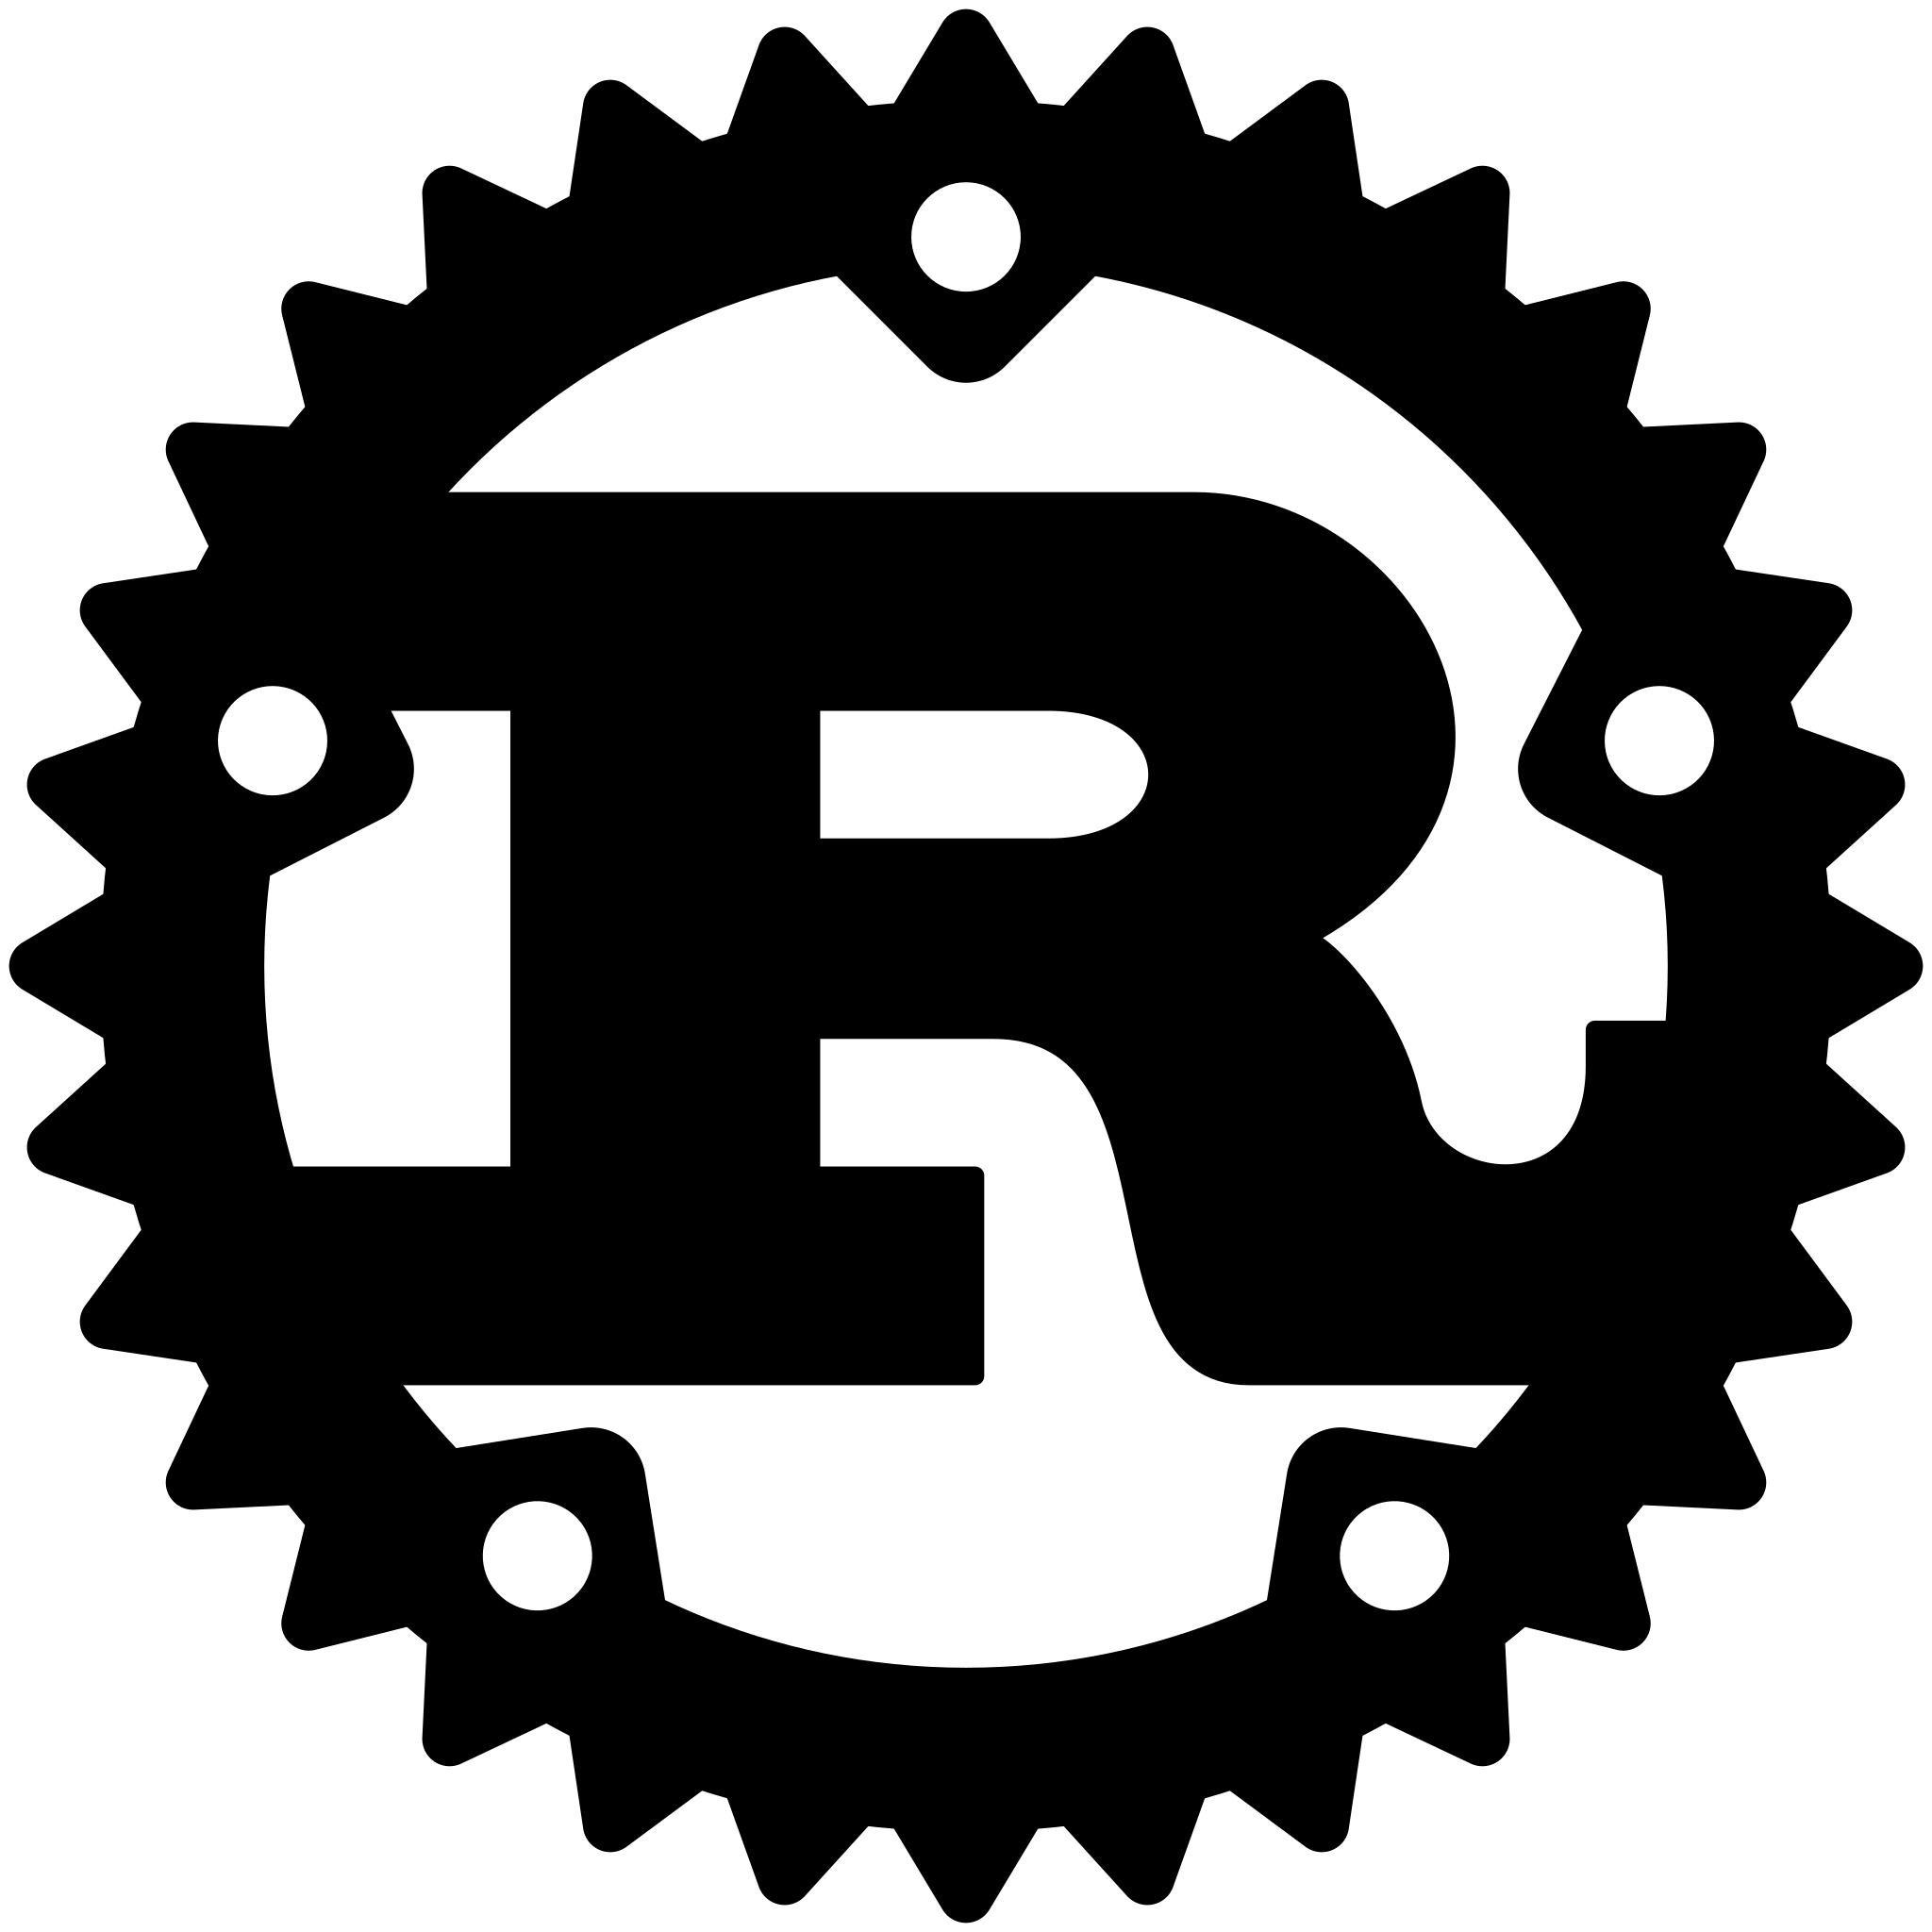
\includegraphics[width=0.25\textwidth]{Images/Rust.png}}
\author{\textit{\textbf{Alireza Lotfi, Alireza Rostami, Sina Amini}}}
\institute[Shiraz Universtiy]
{
	Department of Computer Science, Engineering \& IT \\
	Shiraz University
}
\date{Spring Semester, 2022}

\begin{document}
\begin{frame}[plain,noframenumbering]
  \titlepage
\end{frame}

\begin{frame}{Contribution}
    The general collection of information, and answering of the question 1 to 4 was done by Alireza Lotfi. \\
    The answering of the questions 5 to 13 was done by Alireza Rostami. \\
    The answering of question 14 to 18 was done by Sina Amini. \\
    Besides the general information, each person gathered detailed and nuanced information about their section. \\
    The \LaTeX \, part was carried out by Alireza Rostami and Alireza Lotfi.
\end{frame}

\begin{frame}{Overview}
    \begin{multicols*}{2}
        \tableofcontents
    \end{multicols*}
\end{frame}

\section{Introduction}
    \begin{frame}[plain,noframenumbering]
    	\finalpage{\textcolor{Black}{\LARGE\textbf{Introduction}}}
    \end{frame}
	\begin{frame}{History}
		Rust is a systems programming language designed by \textcolor{red}{Graydon Hoare}, developed at \textcolor{red}{Mozilla research} and targeted at high performance applications. Graydon started working on a new programming language called Rust in 2006. The language was first appeared on \textcolor{red}{July 7, 2010}; 11 years ago.
		~\\Rust's major influences include \textcolor{red}{C++}, \textcolor{red}{Cyclone}, \textcolor{red}{Erlang}, \textcolor{red}{Haskell}, and \textcolor{red}{OCaml}. As an example, Rust's type system supports a mechanism called traits, inspired by type classes in the Haskell language. However, it is interesting to know that \underline{Rust is written in Rust!!}
		~\\According to Stack Overflow\footnote{https://insights.stackoverflow.com/survey/2021\\}, for the sixth-year, Rust is the \underline{most loved language}, while Python is the most wanted language for its fifth-year.
	\end{frame}
	\begin{frame}{Why Rust?}
		\begin{itemize}
			\item[\checkmark] \textbf{Performance:} Rust is blazingly fast and memory-efficient \ul{with no runtime or garbage collector}, it can power performance-critical services, run on embedded devices, and easily integrate with other 
			languages.
			\item[\checkmark] \textbf{Reliability:} Rust’s rich type system and ownership model \ul{guarantee memory-safety and thread-safety} — enabling you to eliminate many classes of bugs at compile-time.
			\item[\checkmark] \textbf{Productivity:} Rust has great documentation, a friendly compiler with useful error messages, and top-notch tooling — an integrated package manager and build tool, smart multi-editor support with auto-
			completion and type inspections, an auto-formatter, and more.
		\end{itemize}
	\end{frame}
	\begin{frame}{Applications}
		Rust is a \textcolor{red}{low-level} programming language with direct access to hardware and memory. You can use Rust to write operation systems or microcontroller applications. Below are some use cases of Rust:
	    \setbeamertemplate{itemize items}[circle]
		\begin{itemize}
			\item \textbf{Command Line:} Whip up a CLI tool quickly with Rust’s robust ecosystem and distribute it with ease.
			\item \textbf{WebAssembly:} Rust compiles to web assembly.
			\item \textbf{Networking:} Predictable performance, Tiny resource footprint, Rock-solid reliability.
			\item \textbf{Embedded:} Targeting low-resource devices regarding need for low-level control without giving up high-level conveniences.
		\end{itemize}
	\end{frame}
	\begin{frame}{Compiling and Running Are Separate Steps}
		Before running a Rust program, you \textcolor{red}{must compile} it using the Rust compiler by entering the \textcolor{red}{\textbf{rustc}} command and passing it the name of your source file.
		~\\Rust is an ahead-of-time compiled language, meaning you can compile a program and give the executable to someone else, and they can run it even without having Rust installed.
		~\\Whether you prefer working with code from the command line, or using rich graphical editors, there’s a Rust integration available for your editor of choice:
		~\\~\\
		\begin{center}
		    \hspace{1cm}
\includegraphics[width=0.1\textwidth]{Images/vim.png}
    		\hspace{1cm}
\includegraphics[width=0.1\textwidth]{Images/intellij.png}
    		\hspace{1cm}
\includegraphics[width=0.1\textwidth]{Images/eclipse.png}
    		\hspace{1cm}
\includegraphics[width=0.1\textwidth]{Images/vscode.png}
		\end{center}
	\end{frame}

\begin{frame}[plain,noframenumbering]
    \finalpage{\textcolor{Black}{\LARGE\textbf{Language Characteristics}}}
\end{frame}

\section{Primitive Data Types}
	\begin{frame}{Primitive Data Types}
		Rust provides access to a wide variety of primitives. A sample includes:
		\begin{enumerate}
			\item \textbf{Scalar Types:}
				\begin{itemize}
					\item signed integers: i8, i16, i32, i64, i128 and isize (pointer size)
					\item unsigned integers: u8, u16, u32, u64, u128 and usize (pointer size)
					\item floating point: f32, f64
					\item char Unicode scalar values like 'a', '$\alpha$' and '$\infty$' (4 bytes each)
					\item bool either true or false
					\item and the unit type (), whose only possible value is an empty tuple: ()
				\end{itemize}
			\item \textbf{Compound Types:}
				\begin{itemize}
					\item arrays like [1, 2, 3]
					\item tuples like (1, true)
				\end{itemize}
		\end{enumerate}
	\end{frame}

\section{Variable Binding}
\begin{frame}[fragile]{Variable Bindings}
	Rust provides type safety via \textcolor{red}{static typing}. Variable bindings can be type annotated when declared. However, in most cases, the \underline{compiler will be able to infer the type} of the variable from the context, heavily reducing the annotation burden.
	\begin{columns}[T]
		\begin{column}{0.6 \textwidth}
            \begin{rustcode}
   fn main() {
        let an_integer: u32 = 1;
        let a_boolean: bool = true;
        let unit = ();
    
        // copy an_integer into copied_integer
        let copied_integer = an_integer;
    
        println!("An integer: {:?}", copied_integer);
        println!("A boolean: {:?}", a_boolean);
        println!("Meet the unit value: {:?}", unit);
    }
            \end{rustcode}
		\end{column}
		\begin{column}{0.4 \textwidth}
			\begin{block}{Output}
				An integer: 1 \\
				A boolean: true \\
				Meet the unit value: ()
			\end{block}
		\end{column}
	\end{columns}
\end{frame}

\section{Scoping}
	\begin{frame}{Scoping (\underline{RAII}, Ownership, Borrowing, Lifetime)}
		Scopes play an important part in \textcolor{red}{ownership}, \textcolor{red}{borrowing}, and \textcolor{red}{lifetimes}. That is, they indicate to the compiler when borrows are valid, when resources can be freed, and when variables are created or destroyed.
		~\\Variables in Rust do more than just hold data in the stack: they also own resources. Rust enforces \textcolor{red}{RAII (Resource Acquisition Is Initialization)}, so \underline{whenever an object goes out of scope}, its destructor is called and its owned resources are freed.
		~\\This behavior shields against resource leak bugs, so you'll never have to manually free memory or worry about memory leaks again
	\end{frame}
	\begin{frame}{Scoping (RAII, \underline{Ownership}, Borrowing, Lifetime)}
		General rules of Rust's Ownership are as below:
		\begin{enumerate}
			\item Because variables are in charge of freeing their own resources, resources can \textcolor{red}{only have \textbf{one owner}}. This also prevents resources from being freed more than once. Note that not all variables own resources (e.g. references).
			\item When doing assignments (let x = y) or passing function arguments by value (foo(x)), the \textcolor{red}{ownership of the resources is \textbf{transferred}}.
			\item After moving resources, the \textcolor{red}{previous owner can no longer be used}. This \textbf{avoids creating dangling pointers}.
		\end{enumerate}
	\end{frame}
	\begin{frame}[fragile]{Scoping (RAII, \underline{Ownership}, Borrowing, Lifetime) - Example}
		\begin{columns}[T]
			\begin{column}{0.5 \textwidth}
                \usemintedstyle{pastie}
                \begin{rustcode}

    fn reverse(str: String) -> String {
        str.chars().rev().collect()
    }
    
    fn main() {
        let str1 = String::from("Hello World");
        let str2 = reverse(str1);
        println!("Reverse of {}: {}", str1, str2);
    }
                \end{rustcode}
			\end{column}
			\begin{column}{0.5 \textwidth}
			    \vspace{1cm}
				\begin{block}{Output}
					error[E0382]: borrow of moved value: `str1`
				\end{block}
			\end{column}
		\end{columns}
	\end{frame}
	\begin{frame}{Scoping (RAII, Ownership, \underline{Borrowing}, Lifetime)}
		Most of the time, we'd like to access data \underline{without taking ownership} over it. To accomplish this, Rust uses a \textcolor{red}{\textbf{borrowing mechanism}}. Instead of passing objects by value (T), objects can be passed by reference (\&T).
		
		~\\The compiler statically guarantees (via its borrow checker) that references always point to valid objects. That is, while references to an object exist, the object cannot be destroyed.
		
		~\\Mutable data can be mutably borrowed using \textcolor{red}{\&mut T}. This is called a \textcolor{red}{\textbf{mutable reference}} and gives read/write access to the borrower.
		
		~\\In contrast, \textcolor{blue}{\&T} borrows the data via an \textcolor{blue}{\textbf{immutable reference}}, and the borrower can read the data but not modify it
	\end{frame}
	\begin{frame}{Scoping (RAII, Ownership, \underline{Borrowing}, Lifetime)}
	    General rules of Rust’s Borrowing are as below:
	    \begin{enumerate}
	        \item Any borrow must last for a scope \underline{no greater than that of the owner}.
	        \item \textcolor{red}{Any number of immutable borrows} (\&T) on a particular resource are allowed .
	        \item Only \textcolor{red}{one mutable borrow} (\&mut T) on particular resource is allowed.
	        \item You may have one or the other of these two kinds of borrows, but \textcolor{red}{not both at the same time}.
	    \end{enumerate}
	\end{frame}
	\begin{frame}[fragile]{Scoping (RAII, Ownership, \underline{Borrowing}, Lifetime) - Example}
		\begin{columns}[T]
			\begin{column}{0.5 \textwidth}
                \begin{rustcode}
    fn reverse(str: &String) -> String {
        str.chars().rev().collect()
    }
        
    fn main() {
        let str1 = String::from("Hello World");
        let str2 = reverse(&str1);
        println!("Reverse of {}: {}", str1, str2);
    }
                \end{rustcode}
			\end{column}
			\begin{column}{0.5 \textwidth}
			    \vspace{1cm}
				\begin{block}{Output}
					Reverse of Hello World: dlroW olleH
				\end{block}
			\end{column}
		\end{columns}
	\end{frame}
	\begin{frame}{Scoping (RAII, Ownership, Borrowing, \underline{Lifetime})}
		A \textcolor{red}{lifetime} is a construct the compiler (or more specifically, its borrow checker) uses \textbf{to ensure all borrows are valid}. Specifically, a variable's lifetime \textcolor{blue}{begins} when it is \textcolor{blue}{created} and \textcolor{orange}{ends} when it is \textcolor{orange}{destroyed}. While lifetimes and scopes are often referred to together, they are not the same.
		
		~\\Take, for example, the case where we borrow a variable via \&. The borrow has a \underline{lifetime} that is determined by where it is declared. As a result, the borrow is valid as long as it ends before the lender is destroyed. However, the \underline{scope} of the borrow is determined by where the reference is used.
	\end{frame}

	\begin{frame}[fragile]{Scoping (RAII, Ownership, Borrowing, \underline{Lifetime}) - Example}
	    \begin{rustcode}
    fn main() {
        let i = 3; // Lifetime for `i` starts.
        {
            let borrow1 = &i; // `borrow1` lifetime starts.
            println!("borrow1: {}", borrow1);                    
        } // `borrow1 ends.

        {
            let borrow2 = &i; // `borrow2` lifetime starts.
            println!("borrow2: {}", borrow2);
        } // `borrow2` ends.
    }   // Lifetime ends.
        \end{rustcode}
	\end{frame}

	\section{Enumeration}
	\begin{frame}{Enumeration (Enum)}
	    An enumeration type is a special data type that enables for a variable to be a set of predefined constants. The variable must be equal to one of the values that have been predefined for it.
	    Common examples include compass directions (values of NORTH, SOUTH, EAST, and WEST) and the days of the week.\\ \\
	    Enums are a feature in many languages, but their capabilities differ in each language.\\
	    Rust’s enums are most similar to algebraic data types in functional languages, such as F\#, OCaml, and Haskell.\\ \\
	    The \textcolor{red}{enum} keyword allows the creation of a type which may be one of a few different variants. Any variant which is valid as a  \textcolor{red}{struct} is also valid as an  \textcolor{red}{enum}.
	\end{frame}
	\begin{frame}[fragile]{Enumeration (Enum) - Example}
	    \begin{rustcode}
// Defining an enum.
enum WebEvent {
    // An `enum` may either be `unit-like`, or tuple structures, or c-like structures.
    PageLoad, // unit-like
    PageUnload, // unit-like
    KeyPress(char), // tuple structures
    Paste(String), // tuple structures
    Input(i32, i32, i32), //tuple structures
    Click { x: i64, y: i64 }, // c-like structures
}
        \end{rustcode}
    \end{frame}
    \begin{frame}[fragile]{Enumeration (Enum) - Example}
	    \begin{rustcode}
// A function which takes a `WebEvent` enum as an argument.
fn inspect(event: WebEvent) {
    match event {
        WebEvent::PageLoad => println!("Page loaded."),
        WebEvent::PageUnload => println!("Page unloaded."),
        WebEvent::KeyPress(c) => println!("Pressed character '{}'.", c),
        WebEvent::Paste(s) => println!("Pasted string \"{}\".", s),
        WebEvent::Input(a, b, c) => println!("Inputted {}, {}, {}.", a, b, c),
        WebEvent::Click{x, y} => { println!("Clicked at x={}, y={}.", x, y); },
    }
}
        \end{rustcode}
    \end{frame}
    \begin{frame}[fragile]{Enumeration (Enum) - Example}
	    \begin{columns}[T]
			\begin{column}{0.5 \textwidth}
                \begin{rustcode}
// Let's see some examples!
fn main() {
    let load = WebEvent::PageLoad;
    let unload = WebEvent::PageUnload;
    let pressed = WebEvent::KeyPress('x');
    let pasted = WebEvent::Paste("test".to_owned());
    let input = WebEvent::Input(30, 10, 20);
    let click = WebEvent::Click { x: 20, y: 80 };
    
    inspect(load);
    inspect(unload);
    inspect(pressed);
    inspect(pasted);
    inspect(input);
    inspect(click);
}
        \end{rustcode}
        \end{column}
        \begin{column}{0.5 \textwidth}
			\vspace{3cm}
			\begin{block}{Output}
				Page loaded. \\
				Page unloaded. \\
				Pressed character 'x'. \\
                Pasted string "test". \\
                Inputted 30, 10, 20. \\
                Clicked at x=20, y=80. \\
			\end{block}
		\end{column}
    \end{columns}
	\end{frame}
	\begin{frame}[fragile]{Enum Alias}
	    If you use a \textcolor{red}{type alias}, you can refer to each enum variant via its alias. This might be useful if the enum's name is too long or too generic, and you want to rename it. \\
        \begin{rustcode}
enum VeryVerboseEnumOfThingsToDoWithNumbers {
    Add,
    Subtract,
}

// Creates a type alias
type Operations = VeryVerboseEnumOfThingsToDoWithNumbers;

fn main() {
    // We can refer to each variant via its alias, not its long and inconvenient name.
    let x = Operations::Add;
}
        \end{rustcode}
	\end{frame}
	\begin{frame}[fragile]{Enum Alias - Continued}
	    The most common place you'll see this is in \textcolor{red}{impl} blocks using the \textcolor{red}{self} alias. \\
        \begin{rustcode}
enum VeryVerboseEnumOfThingsToDoWithNumbers {
    Add,
    Subtract,
}

impl VeryVerboseEnumOfThingsToDoWithNumbers {
    fn run(&self, x: i32, y: i32) -> i32 {
        match self {
            Self::Add => x + y,
            Self::Subtract => x - y,
        }
    }
}
        \end{rustcode}
	\end{frame}
	\begin{frame}[fragile]{Enum Operations}
	Rust enumerations are safe; thus, many operations that are legal in C, are illegal here. \\
        \begin{rustcode}
enum Weekends {
    Saturday = 0,
    Sunday,
}

enum Colors {
    Red = 2,
    Blue,
}
   \end{rustcode}
	\end{frame}
\begin{frame}[fragile]{Enum Operations - Continued}
\begin{rustcode}
fn main() {
    let sat = Weekends::Saturday;
    let red = Colors::Red;
    
    if sat == red { // Invalid. }
    if red == Color::Blue { // Valid, but false. }
    let color: Colors = 1; // Invalid.
    let red_plus = red + 1; // Invalid.
    let red_sat = red + sat; // Invalid.
    let red_times_blue = red * Colors::Blue; // Invalid.
    let cast_blue: i32 = Colors::Blue as i32; // Valid, cast_blue = 3.
    let cast_sat: i32 = sat as i32; // Valid. cast_sat = 0;
}
        \end{rustcode}
	\end{frame}
	
	\begin{frame}[fragile]{Enum as Null}
	    Unlike many languages, Rust does not have a \textcolor{red}{Null} value! Instead, it uses something called \textcolor{red}{Option}. \\
	    Type \textcolor{red}{Option} represents an optional value; every \textcolor{red}{Option} is either \textcolor{red}{Some} and contains a value, or \textcolor{red}{None}, and does not. \textcolor{red}{Option} types are very common in Rust. \\
	    \begin{rustcode}
enum Option<T> {
   Some(T),
   None,
}
        \end{rustcode}
	\end{frame}
	\begin{frame}[fragile]{Enum as Null - Example}
	    \begin{columns}
	    \begin{column}{0.6 \textwidth}
            \begin{rustcode}
fn logarithm (arg: f64, base: f64) -> Option<f64> {
    if base == 0.0 || base == 1.0 { None }
    else { Some(arg.log(base)) }
}
fn main() {
    let res_1: Option<f64> = logarithm(10.0, 2.0);
    match res_1 {
        Some(x) => println!("Result: {}", x),
        None => println!("Log with base 0 and 1 is not defined."),
    }
    let res_2: Option<f64> = logarithm(10.0, 1.0);
    match res_2 {
        Some(x) => println!("Result: {}", x),
        None => println!("Log with base 0 and 1 is not defined."),
    }
}
        \end{rustcode}
    \end{column}
	\begin{column}{0.4 \textwidth}
		\vspace{-3cm}
		\begin{block}{Output}
		Result: 3.3219280948873626 \\
        Log with base 0 and 1 is not defined.
		\end{block}
	\end{column}
    \end{columns}
    \end{frame}
\begin{frame}[fragile]{Enum as Exception}
	    Similar to Option, there is something called Result. Rust does not have exceptions. Instead, it has the type Result<T, E> for recoverable errors and the panic! macro that stops execution when the program encounters an unrecoverable error. \\
	    Type Result is the type used for returning and propagating errors. It is an enum with the variants, Ok(T), representing success and containing a value, and Err(E), representing error and containing an error value.
	    \begin{rustcode}
enum Result<T, E> {
   Ok(T),
   Err(E),
}
        \end{rustcode}
	\end{frame}
	\begin{frame}[fragile]{Enum as Exception - Example}
	        \begin{rustcode}
use std::fs::File;
fn main() {
    let file_opened: Result<File> = File::open("test.txt");
    match file_opened {
        Ok(_file) => let file: File = _file,
        Err(_error) => panic!("Could not open file. Faced error: {:?}", _error),
    }
}
        \end{rustcode}
    \end{frame}

\section{Associative Arrays}
\begin{frame}[fragile]{Associative Arrays (Hash Maps)}
	    Associative arrays are used to represent collections of data elements that can be retrieved by specifying a name called a key. \\
	    In Rust, associative arrays are called hash maps. \\
        The type \textcolor{red}{HashMap <K, V>} stores a mapping of keys of type K to values of type V.
\end{frame}
	\begin{frame}[fragile]{Associative Arrays (Hash Maps) - Example}
	        \begin{rustcode}
use std::collections::HashMap;
let mut book_reviews: HashMap<&str, &str> = HashMap::new();

// Review some books.
book_reviews.insert("Adventures of Huckleberry Finn".to_string(), "My favorite book.".to_string());
book_reviews.insert("Grimms' Fairy Tales".to_string(), "Masterpiece.".to_string());
book_reviews.insert("Pride and Prejudice".to_string(), "Very enjoyable.".to_string());
book_reviews.insert("The Adventures of Sherlock Holmes".to_string(), "Eye lyked it alot.".to_string());
book_reviews.insert("The Art of War".to_string(), "Informative.".to_string());
book_reviews.insert("Crime and Punishment".to_string(), "Fascinating.".to_string());
book_reviews.insert("The Tell-Tale Heart".to_string(), "Horrifying.".to_string());
        \end{rustcode}
    \end{frame}

\begin{frame}[fragile]{Associative Arrays (Hash Maps) - Example}
	       \begin{rustcode}
// Check for a specific book.
let _book = "Les Misérables";
if !book_reviews.contains_key(_book) {
    println!("{} is not in our database.", _book);
}

// Delete an entry.
book_reviews.remove("The Adventures of Sherlock Holmes");

// Look up the values associated with some keys.
let to_find = ["Pride and Prejudice", "Alice's Adventure in Wonderland"];
for &book in &to_find {
    match book_reviews.get(book) {
        Some(review) => println!("{book}: {review}"),
        None => println!("{book} is unreviewed.")
    }
}
\end{rustcode}
    \end{frame}

\begin{frame}[fragile]{Associative Arrays (Hash Maps) - Example}
	        \begin{rustcode}
// Look up the value for a key (will panic if the key is not found).
println!("Review for Jane: {}", book_reviews["Pride and Prejudice"]);

// Iterate over everything.
for (book, review) in &book_reviews {
    println!("{book}: \"{review}\"");
}

        \end{rustcode}
    \end{frame}
    \begin{frame}[fragile]{Associative Arrays (Hash Maps) - Example}
    A hash map with a known list of items can be initialized from an array. \\
	        \begin{rustcode}
use std::collections::HashMap;
let courtesy_names = HashMap::from([
    ("Cao Cao", "Mengde"),
    ("Liu Bei", "Xuande"),
    ("Zhuge Liang", "Kongming"),
    ("Guan Yu", "Yunchang"),
    ("Yuan Shao", "Benchu")
]);

        \end{rustcode}
    \end{frame}
\section{Union}
\begin{frame}[fragile]{Union}
	    Union is a data type that allows different data types to be stored in the same memory locations. Union provides an efficient way of reusing the memory location, as only one of its members can be accessed at a time. \\
	    The size of a union is determined by the size of its largest field. \\ \\
	    Rust is influenced by C/C++, so it supports unions \underline{BUT ONLY IN UNSAFE MODE}. \\\\ A union is defined as follows:
	    \begin{rustcode}
union TestUnion {
    data_integer64: i64,
    data_float64: f64,
    data_unsigned32: u32
}
\end{rustcode}
\end{frame}
	\begin{frame}[fragile]{Union - Continued}
	With no additional checking and lack of discrimination, unions in Rust are free!\\
    As a language that reliability is its top priority, Rust cannot guarantee safety of accessing unions in safe mode; thus, one cannot access unions fields directly. \\
    As result, unions are only accessiable in unsafe mode. \\
When one uses unsafe mode, one takes full responisbility from the compiler for any problems, resulting in highering the chances of failure, which in turns results in undefined behavior.
	        \begin{rustcode}
union TestUnion {
    data_integer64: i64, data_float64: f64, data_unsigned32: u32
}
fn main() {
    let test = TestUnion {data_unsigned32: 1};
    let f = unsafe {test.data_unsigned32};
    println!("{}", f); // Prints: 6
    let f = unsafe {test.data_float64};
    println!("{}", f); // Undefined Behavior
}
        \end{rustcode}
    \end{frame}

\section{Garbage Collection}
\begin{frame}[fragile]{Garbage Collection}
	    Garbage collection is a form of automatic memory management. The garbage collector attempts to reclaim memory which was allocated by the program, but is no longer referenced—also called as garbage. \\ There are two major methods for garbage collection:
	    \setbeamertemplate{itemize items}[circle]
	    \begin{itemize}
	        \item Reference Counting
	        \item Mark and Sweep
	    \end{itemize}

	    Rust does not use any of these methods. Rust has a static garbage collector.\\
        Rust uses \textcolor{red}{Ownership} rules we previously addressed. Rust would know when the variable gets out of scope or its lifetime ends at compile time and thus insert the corresponding LLVM/assembly instructions to free the memory.
\end{frame}

\section{Function}
\begin{frame}[fragile]{Function}
	    Functions are declared using the \textcolor{red}{fn} keyword. Its arguments are type annotated, just like variables, and, if the function returns a value, the return type must be specified after an arrow \textcolor{red}{->}. \\ \\
        The final expression in the function will be used as return value. Alternatively, the \textcolor{red}{return} statement can be used to return a value earlier from within the function, even from inside loops or if statements. \\
	   \begin{rustcode}
fn is_divisible_by(lhs: u32, rhs: u32) -> bool {
    // This is a corner case (early return), so we use the `return` keyword.
    if rhs == 0 { return false; }
    // This is an expression, the `return` keyword is not necessary here.
    lhs % rhs == 0
}
        \end{rustcode}

\end{frame}
\begin{frame}[fragile]{Function - Continued}
	 \begin{columns}
	 \begin{column}{0.5 \textwidth}
	        \begin{rustcode}
// Functions that do NOT return a value,
// actually return the unit type `()`.
fn hello_1(name: String) -> () {
    println!("Hello {}", name);
}
fn main() {
    hello_1("World".to_string());
}
        \end{rustcode}
    \begin{block}{Output}
		Hello World
	\end{block}
    \end{column}
	\begin{column}{0.5 \textwidth}
		    \begin{rustcode}
// When a function returns `()`, 
// the return type can be omitted from the signature.
fn hello_2(name: String) {
    println!("Hello {}", name);
}
fn main() {
    hello_2("World".to_string());
}
        \end{rustcode}
    \begin{block}{Output}
		Hello World
	\end{block}
    \end{column}

    \end{columns}
\end{frame}
\section{Function Parameters}
\begin{frame}[fragile]{Function Parameters: Positional or Keyword?}
	    Rust only supports positional, and does NOT support keyword parameter passing. \\ \\
	   \begin{rustcode}
fn printer(a: &f32, b: u32) {
    println!("The values of float32 a={} and unsigned32 of b={}", a, b);
}
fn main() {
    let a: f32 = 10.0;
    let b: u32 = 5;
    printer(&a, b);
}
        \end{rustcode}
\begin{block}{Output}
The values of float32 a=10 and unsigned32 of b=5
	\end{block}
\end{frame}
\begin{frame}[fragile]{Function Parameters: Builder Pattern}
    Although Rust does not support keyword arguments, such behavior can be implemented using something called \textcolor{red}{Builder pattern}. \\
	       \begin{rustcode}
#[derive(Debug)]
pub enum Align { Left, Center, Right }

#[derive(Debug)]
pub enum Shape { Circle, Square, Triangle }

#[derive(Default)]
pub struct Button {
    label: String,
    align: Option<Align>,
    shape: Option<Shape>,
}
 \end{rustcode}
    \end{frame}

\begin{frame}[fragile]{Function Parameters: Builder Pattern  - Continued}
	       \begin{rustcode}
impl Button {
    pub fn new() -> Button { Default::default() }
    pub fn label(mut self, label: String) -> Button {
        self.label = label; self
    }
    pub fn align(mut self, _align: Option<Align>) -> Button {
        self.align = _align; self
    }
    pub fn shape(mut self, _shape: Option<Shape>) -> Button {
        self.shape = _shape; self
    }
    pub fn desired_function(self) { // We can know define the function we wanted to implement.
        println!("Button {} has shape {:?} and alignment {:?}.", 
            self.label, self.shape.unwrap(), self.align.unwrap()
        );
    }
}
        \end{rustcode}
\end{frame}

\begin{frame}[fragile]{Function Parameters: Builder Pattern - Continued}
Let's see if everything works! \\
	   \begin{rustcode}
fn main() {
    let bt_circ_right = Button::new()
        .shape(Some(Shape::Circle))
        .align(Some(Align::Right))
        .label("Right-Circle-Button".to_string());
    let bt_squ_center = Button::new()
        .label("Center-Square-Button".to_string())
        .shape(Some(Shape::Square))
        .align(Some(Align::Center));
    let bt_tri_left = Button::new()
        .align(Some(Align::Left))
        .label("Left-Triangle-Button".to_string())
        .shape(Some(Shape::Triangle));
 \end{rustcode}
    \end{frame}

\begin{frame}[fragile]{Function Parameters: Builder Pattern - Continued}
	   \begin{rustcode}

    bt_circ_right.desired_function();
    bt_squ_center.desired_function();
    bt_tri_left.desired_function();
}
        \end{rustcode}
\begin{block}{Output}
Button Right-Circle-Button has shape Circle and alignment Right.\\
Button Center-Square-Button has shape Square and alignment Center.\\
Button Left-Triangle-Button has shape Triangle and alignment Left.\\
\end{block}
\end{frame}

\section{Function Defaults}
\begin{frame}[fragile]{Function Parameters: Default Value?}
	    Rust does NOT support keyword parameter passing. But there are some solutions! \\ \\
	    One solution is quite easy. In the previous slides, we talked about pattern building. If we just change the \textcolor{red}{new} function in the implementation, we have achieved default values for functions!
	        The following code is the same as above, just changing the \textcolor{red}{new} function. \\
	   \begin{rustcode}
impl Button {
    pub fn new() -> Button { 
        Button {
            label: "default".to_string(),
            shape: Some(Shape::Circle),
            align: Some(Align::Center),
        }
    }
    ...
}
        \end{rustcode}
\end{frame}
\begin{frame}[fragile]{Function Parameters: Default Value - Continued}
	        \begin{rustcode}
fn main() {
    let defult_button = Button::new();
    let bt_squ_center = Button::new()
        .label("Center-Square-Button".to_string())
        .shape(Some(Shape::Square))
        .align(Some(Align::Center));

    defult_button.desired_function();
    bt_squ_center.desired_function();
}
        \end{rustcode}
\begin{block}{Output}
Button Default-Button has shape Circle and alignment Center. \\
Button Center-Square-Button has shape Square and alignment Center.
\end{block}
\end{frame}

\begin{frame}[fragile]{Function Parameters: Default Value - Continued}
	    Another method is to use \textcolor{red}{Option} and a method called \textcolor{red}{unwrap\_or}.
	   \begin{rustcode}
// Default value of b = 2
fn multiply(a: Option<i32>, b: Option<i32>) -> i32 {
    a.unwrap() * b.unwrap_or(2)
}
fn main() {
    println!("5 times default b is equall to {}.", multiply(Some(5), None));
    println!("5 times 3 is equall to {}.", multiply(Some(5), Some(3)));
}
        \end{rustcode}
\begin{block}{Output}
5 times default b is equall to 10. \\
5 times 3 is equall to 15.
\end{block}
\end{frame}
\section{Function Variadic Arguments}
\begin{frame}[fragile]{Function: Variable Number of Parameters?}
	    Rust does NOT support variadic functions, except when inter-operating with C code that uses varargs. But like other topics we discussed, there are some ways to implement this. \\ \\
	    One solution is quite easy. We again can use \textcolor{red}{Pattern building}, to achieve variadic functions!
	    Let's write an example for the \textcolor{red}{Button} problem.\\
	   \begin{rustcode}
impl Button {
    pub fn new() -> Button { Default::default() }
    ...
    pub fn desired_function(self) { // We can know define the function we wanted to implement.
        match self.shape {
            Some(x) => println!("Button {} has shape {:?}.", self.label, x),
            None => println!("Button {} does NOT have a shape.", self.label),
        }
    }
}
        \end{rustcode}
\end{frame}
\begin{frame}[fragile]{Function: Variable Number of Parameters? - Continued}
	        \begin{rustcode}
fn main() {
    let bt_circ_right = Button::new()
        .shape(Some(Shape::Circle))
        .align(Some(Align::Right))
        .label("Right-Circle-Button".to_string());
    let bt_center = Button::new()
        .label("Center-Button".to_string())
        .align(Some(Align::Center));
    bt_circ_right.desired_function();
    bt_center.desired_function();
}
        \end{rustcode}
\begin{block}{Output}
Button Right-Circle-Button has shape Circle. \\
Button Center-Button does NOT have a shape.
\end{block}
\end{frame}
\begin{frame}[fragile]{Function: Variable Number of Parameters? - Continued}
    If variables are of the same type, we can also use arrays.\\
	       \begin{rustcode}
fn printer(args: &[&str]) {
    for arg in args {
        println!("{}", arg);
    }
}
fn main() {
    printer(&["Rust implementation", "of", "variadic functions."]);
}
        \end{rustcode}
\begin{block}{Output}
Rust implementation \\
of \\
variadic functions.
\end{block}
\end{frame}
\begin{frame}[fragile]{Function: Variable Number of Parameters? - Continued}
    One slightly harder solution is \textcolor{red}{calculate\!} macro.
	   \begin{rustcode}
macro_rules! print_all {
    ($($args:expr),*) => {{
        $( println!("{}", $args); )*
    }}
}
fn main() {
    let a: u32 = 1; let b: i32 = 2; let c: f64 = 3.1; let d: String = "Hello".to_string();
    print_all!(a, b, c, d);
}

        \end{rustcode}
\begin{block}{Output}
1\\
2\\
3.1\\
Hello\\
\end{block}
\end{frame}

\section{Parameter Passing}
\begin{frame}[fragile]{Function Parameter Passing: Call–by–value?}
	    Rust supports call–by–value parameter passing. \\
	   \begin{rustcode}
fn times2(n_loc: i64) -> i64 {
    n_loc * 2
}
fn main() {
    let n_main: i64 = 5;
    println!("{}", times2(n_main));
}
    \end{rustcode}
\begin{block}{Output}
10
\end{block}
\end{frame}
\begin{frame}[fragile]{Function Parameter Passing: Call–by–value-result?}
	   \textcolor{red}{Rust does NOT support call–by–value-result parameter passing.}
\end{frame}
\begin{frame}[fragile]{Function Parameter Passing: Call–by–result?}
	   \textcolor{red}{Rust does NOT support call–by–result parameter passing.}
\end{frame}
\begin{frame}[fragile]{Function Parameter Passing: Call–by–reference?}
	   Rust supports call-by-reference. It achieves such behavior by passing the access path (pass-by-sharing). \\
	   \begin{rustcode}
fn times2(n_loc: &mut i64) -> () {
    *n_loc *= 2
}
fn main() {
    let mut n_main: i64 = 5;
    times2(&mut n_main);
    println!("{}", n_main);
}

    \end{rustcode}
\begin{block}{Output}
10
\end{block}
\end{frame}

\begin{frame}[fragile]{Function Parameter Passing: Call–by-name?}
	   \textcolor{red}{Rust does NOT support call–by-name parameter passing.}
\end{frame}

\section{Function Overloading}
    \begin{frame}[fragile]{Function Overloading}
        Rust \textcolor{red}{does NOT support} overloaded functions/methods. Usually you make separate functions foo(), foo\_mut(), try\_foo(), foo\_with\_bar().
        
        ~\\For some specific usages, it is possible to give overload-like interface using something called a \textcolor{red}{trait}, which is similar to Java's interface. For example, to accept any type that is string-like, one could use:\\
        \begin{rustcode}
fn foo(s: impl AsRef<str>) {s.as_ref()}
// or
fn foo(s: impl Into<String>) {s.into()}
        \end{rustcode}
    \end{frame}
    \begin{frame}[fragile]{Function Overloading - Continued}
        For comparison, consider the following C++ code to and its equivalent Rust code.\\
        \begin{columns}
    \begin{column}{0.5 \textwidth}
        \begin{minted}[baselinestretch=1.2, style=pastie, fontsize=\footnotesize]{C++}
void print(const int &i) 
{
    std::cout << "Integer " << i << std::endl;
}
void print(const double &f) 
{
    std::cout << "Float " << f << std::endl;
}
void print(const std::string &s) 
{
    std::cout << "String " << s << std::endl;
}
        \end{minted}
    \end{column}
	    \begin{column}{0.5 \textwidth}
        \begin{rustcode}
trait Printable {
    fn print(&self, writer : &io::Write);
}
imp Printable for i32 {
    fn print(&self, writer: &io::Write) { // TODO }
}
imp Printable for f64 {
    fn print(&self, writer: &io::Write) { // TODO }
}
imp Printable for String {
    fn print(&self, writer: &io::Write) { // TODO }
}
        \end{rustcode}
    \end{column}

    \end{columns}

    \end{frame}

\section{Closures}
    \begin{frame}[fragile]{Closures}
        Closures are functions that can capture the enclosing environment. For example, a closure that captures the x variable:
	        \begin{rustcode}
|val| val + x
        \end{rustcode}
        ~\\The syntax and capabilities of closures make them \ul{very convenient for on the fly usage}. Calling a closure is exactly like calling a function. However, both input and return types can be inferred and input variable names must be specified.
        ~\\Other characteristics of closures include:
        \setbeamertemplate{itemize items}[circle]
        \begin{itemize}
            \item Using || instead of () around input variables.
            \item Optional body delimination ({}) for a single expression (\ul{mandatory otherwise}).
            \item The ability to capture the outer environment variables.
        \end{itemize}
    \end{frame}
    
    \begin{frame}[fragile]{Closures - Example}
        \begin{columns}[T]
			\begin{column}{0.6 \textwidth}
    	        \begin{rustcode}
fn main() {
    // Increment via closures and functions.
    fn function(i: i32) -> i32 { i + 1 }

    // Closures are anonymous
    // Here we are binding them to references
    let closure_annotated = |i: i32| -> i32 { i + 1 };
    let closure_inferred  = |i     |          i + 1  ;

    println!("function: {}", function(1));
    println!("closure_annotated: {}", closure_annotated(1));
    println!("closure_inferred: {}", closure_inferred(1));

    // A closure taking no arguments which returns an `i32`.
    let one = || 1;
    println!("closure returning one: {}", one());}
                \end{rustcode}
			\end{column}
			\begin{column}{0.4 \textwidth}
				\begin{block}{Output}
					function: 2\\
                    closure\_annotated: 2\\
                    closure\_inferred: 2\\
                    closure returning one: 1
				\end{block}
			\end{column}
		\end{columns}
    \end{frame}

    \begin{frame}{Closures: As Input Parameters}
        While Rust chooses how to capture variables on the fly mostly without type annotation, this ambiguity is not allowed when writing functions. 
        ~\\When taking a closure as an input parameter, the closure's complete type must be annotated using one of a few traits, and they're determined by what the closure does with captured value. 
        In order of decreasing restriction, they are:
        \setbeamertemplate{itemize items}[circle]
        \begin{itemize}
            \item \textbf{Fn:} the closure uses the captured value by reference \textcolor{red}{(\&T)}
            \item \textbf{FnMut:} the closure uses the captured value by mutable reference \textcolor{red}{(\&mut T)}
            \item \textbf{FnOnce:} the closure uses the captured value by value \textcolor{red}{(T)}
        \end{itemize}
        ~\\Moreover, if you declare a function that takes a closure as parameter, then any function that satisfies the trait bound of that closure can be passed as a parameter.
    \end{frame}
    \begin{frame}[fragile]{Closures: As Input Parameters - Example}
        \begin{columns}[T]
			\begin{column}{0.6 \textwidth}
                \begin{rustcode}
// Define a function which takes a generic `F` argument
// bounded by `Fn`, and calls it
fn call_me<F: Fn()>(f: F) {
    f();
}
// Define a wrapper function satisfying the `Fn` bound
fn function() {
    println!("I'm a function!");
}
fn main() {
    // Define a closure satisfying the `Fn` bound
    let closure = || println!("I'm a closure!");

    call_me(closure);
    call_me(function);
}
                \end{rustcode}
			\end{column}
			\begin{column}{0.4 \textwidth}
				\begin{block}{Output}
					I'm a closure!\\
                    I'm a function!
				\end{block}
			\end{column}
		\end{columns}
    \end{frame}

\section{Pass Functions to Function}
    \begin{frame}[fragile]{Pass Functions to Function (Function Pointer)}
        We can also pass regular functions to functions! This technique is useful when you want to pass a function you’ve already defined rather than defining a new closure. Doing this with function pointers will allow you to use functions as arguments to other functions. Functions coerce to the type fn (with a lowercase f), not to be confused with the Fn closure trait. \ul{The fn type is called a function pointer}.
        \begin{columns}[T]
			\begin{column}{0.6 \textwidth}
               \begin{rustcode}
fn add_one(x: i32) -> i32 {
    x + 1
}
fn do_twice(f: fn(i32) -> i32, arg: i32) -> i32 {
    f(arg) + f(arg)
}
fn main() {
    let answer = do_twice(add_one, 5);
    println!("The answer is: {}", answer);
}
                \end{rustcode}
			\end{column}
			\begin{column}{0.4 \textwidth}
				\begin{block}{Output}
					The answer is: 12
				\end{block}
			\end{column}
		\end{columns}
    \end{frame}
    
\section{Coroutine (Generators)}
    \begin{frame}{Coroutine}
        The generators feature gate in Rust allows you to define generator or coroutine literals. A generator is a "resumable function" that syntactically resembles a closure but compiles to much different semantics in the compiler itself. 
        
        ~\\Generators use the \textcolor{red}{yield} keyword to \textcolor{red}{"return"}, and then the caller can resume a generator to \textcolor{blue}{resume execution} just after the \textcolor{blue}{yield} keyword. 
        
        ~\\Generators are an extra-unstable feature in the compiler right now. Added in RFC 2033 they're mostly intended right now as a information/constraint \ul{gathering phase}. The intent is that experimentation can happen on the \ul{nightly compiler} before actual stabilization. 
    \end{frame}
    
    \begin{frame}[fragile]{Coroutine (Generators) - Example}
        \begin{columns}[T]
			\begin{column}{0.6 \textwidth}
                \begin{rustcode}
#![feature(generators, generator_trait)]
use std::ops::Generator;
use std::pin::Pin;
fn main() {
    let mut generator = || {
        println!("2");
        yield;
        println!("4");
    };
    println!("1");
    Pin::new(&mut generator).resume(());
    println!("3");
    Pin::new(&mut generator).resume(());
    println!("5");
}
                \end{rustcode}
			\end{column}
			\begin{column}{0.4 \textwidth}
				\begin{block}{Output}
					1\\
                    2\\
                    3\\
                    4\\
                    5
				\end{block}
			\end{column}
		\end{columns}
    \end{frame}

\begin{frame}[plain,noframenumbering]
    \finalpage{\textcolor{Black}{\LARGE\textbf{References}}}
\end{frame}

\section{References}
	\begin{frame}[allowframebreaks]{References}
		\nocite{*}
		\bibliographystyle{unsrt}
		\bibliography{Bibliography}
	\end{frame}

\end{document} 